\section{Discussion}
\setlength{\parindent}{10ex}
This chapter explores the interesting concepts and emergent ideas that stem from this work.
It is divided into discussing the three core experiments performed.
Specifically, discussing concepts from the regression, classification, and novel grid optimization experiments.

\subsection{Regression Discussion}
\cite{jena2012prediction} achieved a \ac{RMSE} of \~{}175m in their optimized model.
Their model used \ac{ML} to predict a optimum scaling factor S.
The linear regression model fit in this project is 100 meters less accurate than the optimized model used in \cite{jena2012prediction}.
The purpose of the test is not to achieve accurate predictions, but to identify if \ac{ML} models can be viable for predictin bathymetry.
Therefore, the accuracy of these models is less important than identifying the viability of the models.
The training data used is predicted bathymetry, but shows that fitting a model to true bathymetry will yield a similar result.
In any event, the accuracy of these regression models is not viable for true models.

\subsection{Classification Results Discussion}
The Random Forest model performed excellently with a balanced accuracy of 82\%.
Breaking down the results by class, the classifier predicted some classes with greater precision than others.
This is indicative that the decision boundary responded to certain trends in the data.
This can be seen in figure \ref{fig:rfc_report}.

\begin{figure}[htb]
    \centering
    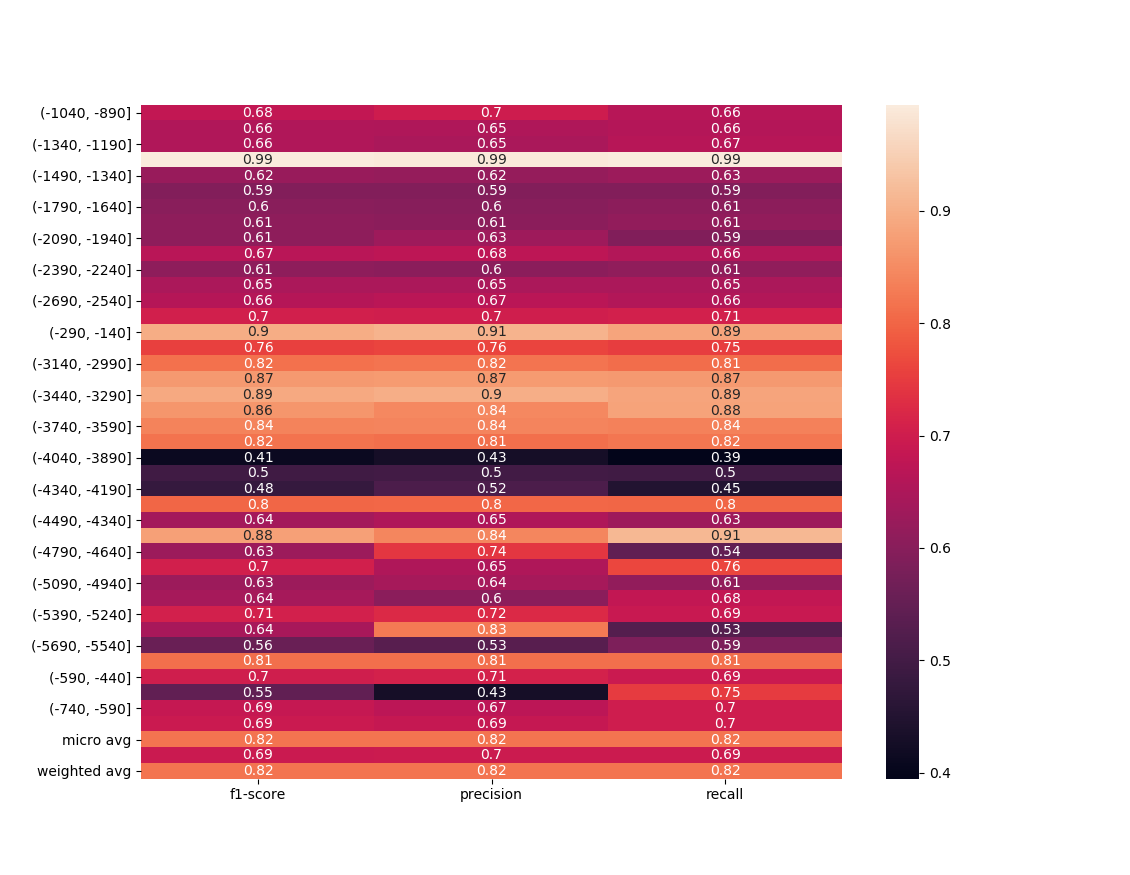
\includegraphics[width=\textwidth]{rfc_class_report.png}
    \caption{Figure displaying the heat map classification report of the Random Forest Classifier}
    \label{fig:rfc_report}
\end{figure}

\par
The Bagging classifier performed on par with the Random Forest Classifier with a balanced accuracy of 79\%.
However, Figure \ref{fig:coveragegrid} shows that the bagging classifier performed best around coastlines.
This suggests the the model responds well to shallow waters.
Shoreline data will also be consistently more accurate because of proximity to land.
Most of the world high resolution bathymetry is shoreline, and it is possible that the model responded to the quality data.


\par
Classification shows that labeling bathymetry can improve the performance of the models.
Being that a random forest model can predict 82\% of the world's predicted bathymetry within 150 meters of accuracy. 
However, what is more interesting to analyze is the behavior of the models.
The data used in training comes from aggregated external datasets and a predicted bathymetry dataset.
The predictions of these models is being compared to predicted bathymetry which represents the accuracy with relation to predicted values.
Meaning that the accuracy in these models is not indicative of truly predicting global bathymetry.
It does show that a \ac{ML} model can be fit to data and used to predict bathymetry, and if actual measured bathymetry and ocean features were used in training the results would be comparable.
Furthermore, parameter tuning, model selection, and dynamic feature selection could be used the increase the accuracy beyond current results.

\par
Interestingly, some models perform extremely well along fault lines.
For example, the decision tree classifier in figure \ref{fig:coveragegrid} performs extremely well along fault lines.
However, when making predictions in the global scope the classifier is very inaccurate.
This suggestions that a classifiers can be optimized by geopatial position.



\subsection{Grid Optimized Model Discussion}
%The world wide ETOPO bathymetry dataset \cite{national1988etopo} at two minute resolution is used for valadation and metrics.
%This dataset is treated as the ground truth for all predictions.
%During the experiment, a one third holdout was used for validation in some cases.
%For finding the optimum model for a coverage a 10 fold cross validation was utilized.

%Include metrics information here.... possibly graphs and a list of scores? I dont really know.

%I dont like how I worded this whole section...
%The idea here is that I want to say "Hey, these people did this research and found the their regression model preforms poorly for predicting seamounts espicially after 500m.
%I clearly noticed a similar trend, but saw better preformance from some models than others. 
%This research is to identify those coverages and then use those results to build a super classifier.
%These metrics are important for identifying where the models preform well. 
\par
The Grid Optimized Model Injector improved the accuracy of predictions by \~{}5\%.
These results are displayed in figure \ref{fig:grid_opt_graph}.
Obviously, the model selection and subsequent injection improved the results of this classifier.
Creating a ensemble of many models and selecting them on demand.
This could be caused by geophysical characteristics that benefit one classifier.
For example, in figure \ref{fig:coveragegrid} the Decision Tree classifier preformed best along what appears to be fault lines.
It is possible that the characteristics related to being in proximity to a fault line benefited the models decision boundary. 

\par
Clearly, figure \ref{fig:coveragegrid} provides evidence that model decision boundaries are sensitive to the features based on location.
Leading to the theory that there is not a single best fit model for predicting global bathymetry.
Analysis of figure \ref{fig:coveragegrid} shows interesting consistencies that raise questions about the underlying features.

\begin{figure}[h]
    \centering
    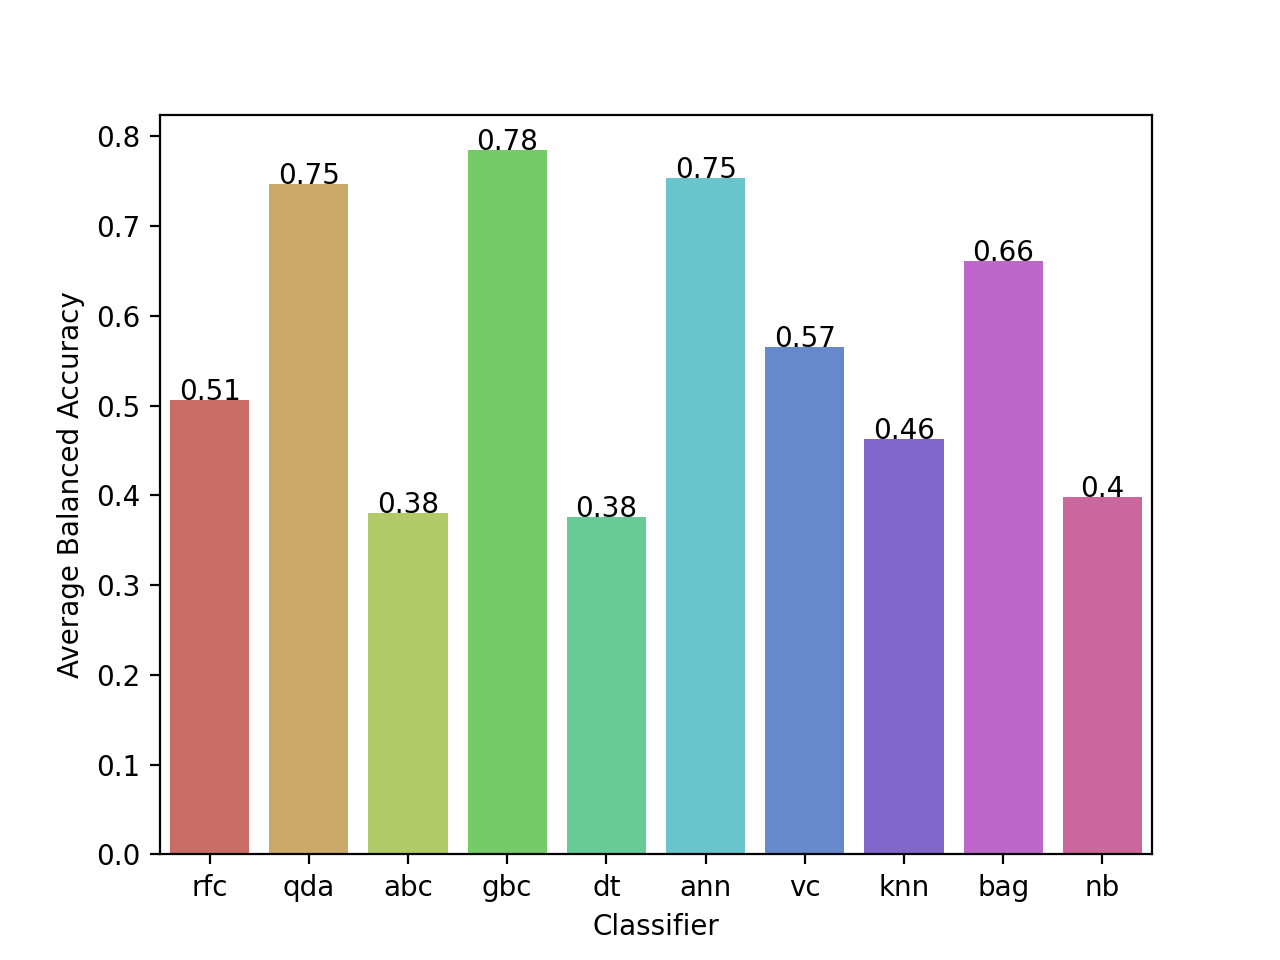
\includegraphics[width=\textwidth]{opt_grid_bar.png}
    \caption{Graph representing the average prediction accuracy of coverages where a model performed well}
    \label{fig:grid_opt_graph}
\end{figure}

\par
Figure \ref{fig:grid_opt_graph} represents the average prediction accuracy across all coverages where a model was "best fit".
What this graph shows is that the Random Forest Classifier had a average prediction rate of 51\% across coverages.
This is fairly consistent with what was expected. 
The models only trained on data contained within a coverage which limited the training and fitting for models. 
However, other models did not suffer from this on average.
This suggestions that some coverages can be larger than others.
For example, coverages where the random forest classifier performed well may yield a higher accuracy if they are decreased or reformed.
Other coverages can be increased in size and potentially yield similar results.

% \begin{table}[htb]
%     \centering
%     \begin{tabular}{|c c c|}
%         \hline
%         \textbf{Model} & \textbf{Average F1 Score} & \textbf{Mean Balanced Accuracy} \\
% 		\hline
% 		Grid Optimized Model Injector & 0.83 & 0.862 \\
% 		\hline
%     \end{tabular}
%     \label{table:GRID_OPT_RESULTS}
%     \caption{Grid Optimized Model Injector Results}
% \end{table}

\par
In any event, there is evidence to support geophysical location drives the factors that help predict bathymetry.
Things to optimize may include investigating the appropriate feature sets, coverage boundaries, depth boundaries, parameters, and metrics based on geophysical location.
For example, volcanic activity creates new land.
This activity has a causal relationship to bathymetry, but volcanic activity at a specific point may not affect the bathymetry at a potential antipodal point.
Another example being that the coverage boundaries are potentially a naive selection choice.
It is possible that choosing models by performance across depth boundaries proves to be a better selector.
%Extending off the research preformed in \cite{jena2012prediction} these metrics allow the selection of the best preforming model.
%This is where I define what happens after the appropriate coverages have been found.
\par
In theory, this injection will allow each model to perform to its optimum.
Each coverage highlights distinct characteristics that will produce a better decision boundary.
These coverages are simple partitions of the world, but could be extended in future work to optimize the selection.
% Reconsider this sentence....



%Maybe here I can have a table show casing the preformance of models or possibly statistics about the coverages??
%It will be intersting to see what has preformed better across the globe
%Also is intersting to see which models have preformed best overall.

\subsection{General Discussion}
The predictions made in this work are based on predicted bathymetry.
Even with a 85\% prediction rate these models are not able to compete with physics models.
The experiments in this work do show that there are accuracy gains to be achieved with model selection.
Figure \ref{fig:coveragegrid} gives incidence that there is not a best fit model for predicting bathymetry globally.
Meaning that a ensemble of some kind combining models based on geospatial location, feature sets, or any other unknown parameter will likely yield better results.

The experiments in this work provide evidence for optimal model selection with regards to predicting global bathymetry.
It is plausible to assume that selecting a model with a decision function will produce better predicitions.
Identifying the optimal decision function will help to explain why different models perform better or worse over a coverage.
This works experimented with a simple geospatial decision function that determined best performing models by previous results.
It was shown to improve the theorectical prediction accuracy.
